\documentclass[usegeometry=true]{scrartcl}
\usepackage[english]{babel}
\usepackage[T1]{fontenc}
\usepackage{lmodern}
\usepackage[utf8]{inputenc}
\usepackage{hyperref}
\usepackage{amssymb}
\usepackage[left=2cm, right=2cm, top=2cm, bottom=2cm, bindingoffset=1cm, includeheadfoot]{geometry} % Don't change dimensions.
\usepackage[onehalfspacing]{setspace} % Don't change spacing.
\usepackage[backend=biber,style=numeric]{biblatex}
\usepackage{csquotes}
\usepackage{relsize}
\usepackage{xcolor}
\usepackage{xspace}
\usepackage{xurl}
\usepackage{listings}
\usepackage{listingsutf8}
\usepackage{booktabs}
\usepackage{tabularx}
\addbibresource{literature.bib}

% Listings
\definecolor{mediumgray}{gray}{0.60}
\definecolor{webiscodebasic}{rgb}{0.2,0.2,0.2}
\definecolor{webiscodekeyword}{rgb}{0.0,0.5,0.0}
\definecolor{webiscodekeywordself}{rgb}{0.7,0.4,0.6}
\definecolor{webiscodeidentifier}{rgb}{0.0,0.0,0.0}
\definecolor{webiscodecomment}{rgb}{0.25,0.5,0.5}
\definecolor{webiscodestring}{rgb}{0.75,0.12,0.12}
\definecolor{webiscodedecorator}{rgb}{0.6,0.3,0.0}
\lstdefinestyle{webisstyle}{
  basicstyle=\ttfamily\color{webiscodebasic},
  keywordstyle=\color{webiscodekeyword},
  identifierstyle=\color{webiscodeidentifier},
  commentstyle=\color{webiscodecomment},
  stringstyle=\color{webiscodestring},
  showstringspaces=false,
  frame=lines,
  framesep=0.7em,
  rulesep=0.5em,
  framerule=0.1em,
  keepspaces=true,
  tabsize=2,
  showtabs=false,
  numbers=none,
  literate=
    {->}{{\textrightarrow}}{2}
    {>=}{{\(\geq\)}}{2}
    {<=}{{\(\leq\)}}{2}
    {!=}{{\(\neq\)}}{2},
}
\lstloadlanguages{Haskell}
\lstset{
  style=webisstyle,
  language=Haskell,
  emph={[1]def,class},
  emphstyle={[1]\color{webiscodekeyword}\bfseries},
  emph={[2]self,cls},
  emphstyle={[2]\color{webiscodekeywordself}},
  emph={[3]@dataclass},
  emphstyle={[3]\color{webiscodedecorator}},
}

% Itemization:
\newcommand{\Ni}{(1)~}
\newcommand{\Nii}{(2)~}
\newcommand{\Niii}{(3)~}
\newcommand{\Niv}{(4)~}
\newcommand{\Nv}{(5)~}
\newcommand{\Na}{(a)~}
\newcommand{\Nb}{(b)~}
\newcommand{\Nc}{(c)~}
\newcommand{\Nd}{(d)~}
\newcommand{\Ne}{(e)~}

% Editing:
\newcommand{\todocite}{{\smaller\color{red}[CITE]}\xspace}
\newcommand{\todo}[1]{{\smaller\color{red}[#1]}}

\begin{document}

\subject{Project Report for the Module \\ \textquote{Information Retrieval und Visualisierung} \\ in Summer Semester~2022}
\title{Insights Towards Safer Roads}
\subtitle{Visualizing Accidents in France from~2005 to~2020}
\author{Jan Heinrich Reimer}
\date{\today}
\maketitle

\tableofcontents
\section{Introduction}
\label{introduction}
Despite decades of developing better technology and regulations to avoid road accidents, the global number of accidents is still high~\cite{Who2015}. In~2009, 1.5\,\% of EU citizens\footnote{\url{https://ec.europa.eu/eurostat/databrowser/bookmark/55b45b50-76ac-4cbf-9493-274087bd96fe}} reported injuries caused by road accidents. And even though in recent years the number of road deaths slightly declined in the European Union\footnote{\url{https://ec.europa.eu/eurostat/web/products-eurostat-news/-/DDN-20220511-1}}, in~2020 still 4 out of 100\,000 inhabitants died of road accidents. Among personal factors such as inexperiencedness or loss of control~\cite{RolisonRMF2018}, combusted cities~\cite{AlbalateF2021} and insufficient law enforcement~\cite{Who2015} are commonly cited as reasons behind those high numbers of accidents. Those are, however, factors that are not easy to change. Neither can urbanization be stopped nor can we circumvent all personal factors. This report instead seeks to develop new ideas towards road safety by visualizing French governmental open datasets of road accidents\footnote{\url{https://data.gouv.fr/en/datasets/bases-de-donnees-annuelles-des-accidents-corporels-de-la-circulation-routiere-annees-de-2005-a-2019/}} that happend in France in the period from~2005 to~2020. We presume that given France's representativity in Europe---with a population of 68~millions it is the second largest country within the 447~million population of the European Union~\footnote{as of January 1 2022, \url{https://ec.europa.eu/eurostat/databrowser/bookmark/40fd4e5f-3ace-4618-86a5-e9ecfea67ac2}}---some of our conclusions can also be applied to other European countries as well. In our Design Study~\cite{Munzner2008}, we propose new visualizations to explore three different dimensions that could cause road accidents: \Ni date- or time-related effects, \Nii the influence of the drivers and passengers, and \Niii prevalences of different types of accidents.

\subsection{Application Background}
\begin{table}
    \caption{Exemplary questions that should be answered by visualizions of French road accident dataset, with the typical background a person asking that question would likely have.}
    \label{table-questions}
    \begin{tabularx}{\linewidth}{Xp{0.3\linewidth}}
        \toprule
        \textbf{Question} & \textbf{Background} \\
        \midrule
        Are roads more dangerous in winter or summer? & citizen \\
        Do older or younger people drive more safely? & policy maker \\
        Are there geographical hotspots, e.g., in cities or rural areas? & citizen, policy maker \\
        If geographical hotspots occur, which other characteristics can explain the correlations. & policy maker \\
        Do the proportion of dead and injured persons correlate? & policy maker \\
        Where are unproportionately more people killed in traffic? & policy maker \\
        Do dedicated bicycle lanes make roads safer for cyclists? & citizen, policy maker, infrastructure planner \\
        Are wider roads safer than narrow roads? & citizen, infrastructure planner \\
        \bottomrule
    \end{tabularx}
\end{table}
With unacceptably high casualties in road traffic, our vizualization addresses the international initiative towards better road safety. The vizualizations should support people in avoiding particuarly dangerous regions, times, or other patterns. It should also provide officials with insights where additional policies or infrastructure might mitigate high numbers of traffic accidents. It is therefore important that broad trends can be expolored while at the same time giving the targetted users the option to dive into visualizations to gain insights on smaller details.
Specifically, our visualizations should answer the following exemplary questions listed in Table~\ref{table-questions}.

\subsection{Target Groups}
Our visualizations target citizens that commute on French roads as well as governments throughout the world. For the first group in particuar, we can not assume deep knowledge of public infrastructure or mechanical vocabulary~(e.g.,~they might not be able to intuitively distinguish between vehicles that weigh 1.5~or 3.5~tons). For policy makers on the other hand, we can assume such extended knowledge, assuming they were trained on special fields of public infrastucture. Both groups want to know where, when, and with whom accidents occur most often, that is, they want to explore patterns, citizens because they could then avoid such patterns and government officials because they could target such patterns by introducing laws or building new infrastructure~(e.g.,~a pedestrian bridge at a dangerous road crossing). 

\subsection{Overview and Contributions}
Our contributions are twofold: \Ni we make the French government's accident dataset more accessible by preprocessing, aggregating, and translating the data of 64~individual, French-named data files, and \Ni we develop an application with three interactive visualizations that help citizens as well as politicians in finding frequent dangers across French roads.
Working with highly multidimensional data, we apply patterns such as filtering and aggregation, partitioning into tree hierarchies~\cite{Shneiderman1992}, icon-based stick figure~\cite{PickettG1988} vizualization techniques, and interacive options to select or order specific dimensions of the dataset for each visualization.
We deploy our described visualizations as an interactive online demo\footnote{\url{https://heinrichreimer.github.io/france-accidents/}} and release the visualization code as well as code for preprocessing the open dataset on GitHub\footnote{\url{https://github.com/heinrichreimer/france-accidents}} under an open license.
The insights gianed from the visualizations introduced in this paper can be integrated in future policies and public infrastructure planning. This way roads can be made safer and people's lives can be saved.

\section{Data}
\label{data}
\begin{table}
    \caption{Files with accident data, released by the French government each year~(denoted by \textit{YYYY}), with description of its contents.}
    \label{table-files}
    \begin{tabularx}{\linewidth}{lX}
        \toprule
        \textbf{File Name} & \textbf{Contents} \\
        \midrule
        \textit{caracteristiques-YYYY.csv} & accident characteristics, time, place, etc. \\
        \textit{lieux-YYYY.csv} & accident location, road numbers, road characteristics, lanes etc. \\
        \textit{usagers-YYYY.csv} & persons involved, sex, birth, equipment, etc. \\
        \textit{vehicules-YYYY.csv} & vehicle type, maneuver, hit obstacles \\
        \textit{vehicules-immatricules-baac-YYYY.csv} & not used in this report \\
        \bottomrule
    \end{tabularx}
\end{table}
The French government publicly releases a dataset\footnote{\url{https://data.gouv.fr/en/datasets/bases-de-donnees-annuelles-des-accidents-corporels-de-la-circulation-routiere-annees-de-2005-a-2019/}} of  metadata on road accidents that occurred between~2005 and~2020. This dataset is released yearly and consist of 5~files per year in CSV format~(cf. Table~\ref{table-files}). Excluding one of the files\footnote{The \textit{vehicules-immatricules-baac-YYYY.csv} files are only available from 2010 to 2020.}, we download a total of 64~files for the 16~years considered for our visualizations. As shown in  Table~\ref{table-files}, the dataset feature a variety of dimensions. Many categorical dimensions describe characteristics of the accidents, vehicles, and persons involved. Using the categories we can filter or partition the dataset across multiple dimensions, in order to focus on specific characteristics in the dataset. The involved persons are also characterized regarding injuries and deadliness of the accident, which allows us to measure not only the number of accidents but also how severe each accident was. Similarly, each vehicle and each person involved in the accident is listed, so that we can count how much impact the accident likely had on the society. Crucially for measuring trends across years or months, each accident in the dataset is annotated with a timestamp. We therefore argue that the provided dataset is well suited to answer questions mentioned in Section~\ref{introduction}. Unfortunately, accidents, locations, vehicles, and persons are distributed in separate files. Hence, in our data preprocessing pipeline, we associate locations, vehicles, and persons to their matching accident.

After first attempts to parse and merge the CSV files directly inside the Elm application we decided to implement the data preprocessing in Python instead, as the type safety in Elm makes it complicated to correct errors in the government open data files. For example, CSV files from some years use different separators and even different file encodings. Also, some fields are named differently or use different number formats. In Python such errors are easier to debug and work around. By preprocessing the CSV files we also group persons by their vehicle and vehicles by the accident.Our Python preprocessing is structured in three parsers, for accidents, vehicles, and persons. After parsing, the three lists are grouped and exported. A smaller sample is extracted due to memory constraints when loading the dataset in the web browser.

\paragraph{Parsers}
\begin{listing}
    \lstinputlisting[linerange={17-17,32-36,43-45,48-48,59-59,74-77,110-111},language=Python]{../preprocessing/parse/person.py}
    \caption{Parser module for the CSV file containing person information. Function and constructor abbreviated.}
    \label{listing-data-parser}
\end{listing}
For each of the four data types, characteristics, locations, vehicles, and persons, we implement a parser module as illustrated in Listing~\ref{listing-data-parser}. The parser modules are responsible for opening the corresponding dataset file for the specified year and then reading the CSV records with the correct file encoding and separator. From the CSV records we then extract Python named tuples to improve type-safety for the JSON export. All columns are stripped from surrounding whitespace or illegal special characters~(e.g., the non-breaking space). For categorical columns~(cf. Listing~\ref{listing-data-parser}), we filter out invalid values and then map the values to Python \lstinline[language=Python]{Enum} classes containing the value coding from the French government's dataset description. Floating point values are parsed after correcting the decimal separator. We also split and parse lists of values contained in the CSV columns~(e.g., for the \lstinline[language=]{secu} column specifying safety equipment). For some columns, we also remove prefixes and suffixes~(e.g., for the upstream terminal~\lstinline[language=]{pr1}). The upstream terminal data is particularly difficult to parse because for some years the \lstinline[language=]{pr}~and \lstinline[language=]{pr1}~columns are swapped and need to be corrected. Each parser returns a list of instances of its corresponding named tuple together with the accident ID, vehicle ID, and person number if applicable.

\paragraph{Accident Grouping}
After parsing records of accidents, vehicles, and persons we match the vehicle and person records with the accidents. This is done by grouping persons by their vehicle ID and then associating each group of persons with the corresponding vehicle. Similarly, vehicles~(together with their associated persons) are then grouped by accident ID and then associating the vehicle groups with the matching accident record. This mapping from three different lists of records into a single list of records, containing lists of lists, makes parsing a single accidents easier in the Elm application.

\paragraph{Export and Sampling}
\label{export}
After preprocessing the data, we bundle the accident dataset as static resource, writing one JSON record per line to the exported JSONL file. For the conversion from Python's named tuple types that we modelled for each of the record types~(i.e., accident, vehicle, and person) to JSON, we convert the named tuples to Python \lstinline[language=Python]{Dict} instances which then can be converted to a JSON string using the built in \lstinline[language=Python]{json.dumps} function. Because of the large size of the aggregated dataset~(1065053~accidents/lines or 2~GB disk size), we also derive a smaller subset of the dataset by uniformly sampling 10\,000 random accidents from the whole dataset~(19~MB disk space). This way we extract a dataset that can be used with regular web browsers on common consumer hardware. To account for sampling biases, we test the visualizations with 3~different samples and find no major visual differences across the samples. We therefore assume that the sample dataset is able to sufficiently represent the whole dataset.

\section{Visualizations}
We propose three interactive visualizations by first analysing a set of tasks our application should solve~(cf. Section~\ref{tasks}), and then deriving specific requirements for the included visualizations~(cf. Section~\ref{requirements}). Furhtermore, we discus expressiveness, effectiveness, and appropriateness for each of the three implemented visualizations~(cf. Section~\ref{presentation}) and explain the interactivity of the visualization application~(cf. Section~\ref{interaction}).

\subsection{Analysis of Application Tasks}
\label{tasks}
\begin{table}
    \caption{Exemplary questions that should be answered by visualizions of French road accident dataset, with the typical background a person asking that question would likely have.}
    \label{table-questions}
    \begin{tabularx}{\linewidth}{cXp{0.3\linewidth}}
        \toprule
        \textbf{\#} & \textbf{Question} & \textbf{Background} \\
        \midrule
        1 & Are roads more dangerous in winter or summer? & citizen \\
        2 & Do older or younger people drive more safely? & policy maker \\
        3 & Are there hotspots of accidents in cities or rural areas? & citizen, policy maker \\
        4 & If hotspots occur, which other characteristics can explain the correlations. & policy maker \\
        5 & Do the proportion of dead and injured persons correlate? & policy maker \\
        6 & Where are unproportionately more people killed in traffic? & policy maker \\
        7 & Do dedicated bicycle lanes make roads safer for cyclists? & citizen, policy maker, infrastructure planner \\
        8 & Are wider roads safer than narrow roads? & citizen, infrastructure planner \\
        \bottomrule
    \end{tabularx}
\end{table}
Because of the diverse application background and target groups described in Section~\ref{introduction}, many tasks can be formulated to be answered by data visualizations. To narrow down the tasks, in this report, we propose a set of exemplary questions our visualizations should answer. The questions listed in Table~\ref{table-questions} also specify the most likely background a person asking that question would have. This additional context allows us to fine-tune individual visualizations by assuming background knowledge from the respective target group.
We identify 3~mental models as most important to help people answer the abovementioned questions: \Ni times and dates, \Nii geographical position, \Niii clustering or categorization.
Time and date, for example, are important to identify periodical trends, as required in question~1 in Table~\ref{table-questions}. A time series plot is able to capture the continuity of time and express a single data dimension in relation to time, which is enough for identifying the dangerousness of specific time periods.
Geographical position is crucial for understanding local patterns, as required in questions~3 or~6. While most people are very familiar with using maps as visualization for geographically positioned data, it is often not obvious how to visualize the multiple dimensions of the data points that are displayed on that map. We argue that given the space constraints of a map, the stick figures technique~\cite{PickettG1988} is appropriate because it can display a fixed number of dimensions in small space while observers can still detect patterns across the maps geographical dimensions.
And clustering accident occasions with respect to different categories is needed for comparing how different characteristics might influence road safety, as required in question~7. When working with multidimensional data, like we do with accidents, trees and treemaps~\cite{Shneiderman1992} can be a good visualization to present different, hierarchical categories.

\subsection{Visualization Requirements}
\label{requirements}
We derive 3~main goals that our visualization application should implement: \Ni to identify dangerous regions, times, and situations, \Nii to summarize trends with respect to time and location, and \Niii to offer detailed views where data is aggregated.
Identifying dangerous patterns should be supported by emphasizing road injuries or road deaths at first glance or by showing differences of accidents' characteristics with respect to visual reference points.
Accidents that follow a specific pattern should be distinguishable from other accidents.
Time-based trends should be made visible both in the long term and in the short term. Geographical trends must also include the geographical position but should not over-emphasize it to be effective.
And to avoid losing important details such as outliers, the visualizations should always feature a way to show the data with as little aggregation~(e.g., average, minimum, maximum) as possible, while still not overwhelming observers of the visualization.

\subsection{Visualization Presentation}
\label{presentation}
The visualization application proposed to solve the aforementioned tasks~(cf. Section~\ref{tasks}) consists of three interatively combined visualization pages: \Ni a time series plot to compare the number of accidents or casualties, \Nii a geographical map of icon-based stick figure visualizations, and \Niii a treemap view of hierarchically categorized accidents.

\subsubsection{First Visualization}
\todo{Präsentieren sie die visuellen Abbildungen und Kodierungen der Daten und Interaktionsmöglichkeiten.
Sie müssen begründen, warum und wie gut ihre Designentscheidungen die erstellten Anforderungen erfüllen.
Weiterhin müssen sie begründen, warum die gewählte visuelle Kodierung der Daten für das zu lösenden Problem passend ist.
Typische Argumente würden hier auf Wahrnehmungsprinzipien und Theorie über Informationsvisualisierung verweisen. 
Die besten Begründungen diskutieren explizit die konkrete Auswahl der Visualisierungen im Kontext von mehreren verschiedenen Alternativen. 
Machen Sie hier nicht den Fehler, einfach nur Visualisierung aus den vorgegebenen Bereichen zu diskutieren, weil das in der Regel nicht sinnvoll ist.
Wenn sie sich für einen Scatterplot entschieden haben, ist ein Zeitreihendiagramm in der Regel keine Alternative.
Diskutieren Sie also nicht einfach Zeitreihendiagramme, weil sie in den Anforderungen an das Projekt neben Scatterplots stehen, sondern suchen sie nach echten alternativen Visualisierungen, die zum Aufbau eines vergleichbaren mentalen Modells führen.
Diskutieren Sie die Expressivität und die Effektivität der einzelnen Visualisierungen.}

\subsubsection{Second Visualization}
We use a equirectanguular map projection of france\footnote{\url{https://commons.wikimedia.org/wiki/File:France_location_map-Regions_and_departements-2016.svg}} as the background to the second visualization.
\todo{Präsentieren sie die visuellen Abbildungen und Kodierungen der Daten und Interaktionsmöglichkeiten.
Sie müssen begründen, warum und wie gut ihre Designentscheidungen die erstellten Anforderungen erfüllen.
Weiterhin müssen sie begründen, warum die gewählte visuelle Kodierung der Daten für das zu lösenden Problem passend ist.
Typische Argumente würden hier auf Wahrnehmungsprinzipien und Theorie über Informationsvisualisierung verweisen. 
Die besten Begründungen diskutieren explizit die konkrete Auswahl der Visualisierungen im Kontext von mehreren verschiedenen Alternativen. 
Machen Sie hier nicht den Fehler, einfach nur Visualisierung aus den vorgegebenen Bereichen zu diskutieren, weil das in der Regel nicht sinnvoll ist.
Wenn sie sich für einen Scatterplot entschieden haben, ist ein Zeitreihendiagramm in der Regel keine Alternative.
Diskutieren Sie also nicht einfach Zeitreihendiagramme, weil sie in den Anforderungen an das Projekt neben Scatterplots stehen, sondern suchen sie nach echten alternativen Visualisierungen, die zum Aufbau eines vergleichbaren mentalen Modells führen.
Diskutieren Sie die Expressivität und die Effektivität der einzelnen Visualisierungen.}

\subsubsection{Third Visualization}
\todo{Präsentieren sie die visuellen Abbildungen und Kodierungen der Daten und Interaktionsmöglichkeiten.
Sie müssen begründen, warum und wie gut ihre Designentscheidungen die erstellten Anforderungen erfüllen.
Weiterhin müssen sie begründen, warum die gewählte visuelle Kodierung der Daten für das zu lösenden Problem passend ist.
Typische Argumente würden hier auf Wahrnehmungsprinzipien und Theorie über Informationsvisualisierung verweisen. 
Die besten Begründungen diskutieren explizit die konkrete Auswahl der Visualisierungen im Kontext von mehreren verschiedenen Alternativen. 
Machen Sie hier nicht den Fehler, einfach nur Visualisierung aus den vorgegebenen Bereichen zu diskutieren, weil das in der Regel nicht sinnvoll ist.
Wenn sie sich für einen Scatterplot entschieden haben, ist ein Zeitreihendiagramm in der Regel keine Alternative.
Diskutieren Sie also nicht einfach Zeitreihendiagramme, weil sie in den Anforderungen an das Projekt neben Scatterplots stehen, sondern suchen sie nach echten alternativen Visualisierungen, die zum Aufbau eines vergleichbaren mentalen Modells führen.
Diskutieren Sie die Expressivität und die Effektivität der einzelnen Visualisierungen.}

\subsection{Interaction}
\label{interaction}
\todo{Die präsentierten Visualisierungstechniken müssen interaktiv zu einer Anwendung verknüpft werden.
Die Interaktion mit einer Visualisierung soll in den anderen Visualisierungen zu einer Änderung führen. 
Erklären Sie die möglichen Interaktionen mit den einzelnen Visualisierungen und die möglichen Verknüpfungen zwischen ihnen. Begründen Sie, warum die konkreten Interaktionen umgesetzt wurden und welche Zwecke für die Anwenderinnen mit ihnen unterstützt werden. Begründen Sie ebenfalls, warum sie andere Interaktionsmöglichkeiten nicht umgesetzt haben. Wenn sie keine der geforderten Interaktionen umsetzen, erhalten Sie im gesamten Projekt deutlichen Punktabzug.}

\section{Implementation}
\todo{Beschreiben Sie die Implementierung ihrer Visualisierungs-Anwendung in Elm. Stellen die Gliederung ihres Quellcodes vor. Haben Sie verschiedene Elm-Module erstellt. Was war aufwändig umzusetzen, was ließ sich mit dem vorhanden Code aus den Übungen relativ einfach umsetzen?}

\todo{Wie sieht die Elm-Datenstruktur für das Model aus, in dem die verschiedenen Zustände der Interaktion gespeichert werden können.}

\section{Use Cases}
The three proposed visualizations are evaluated by presenting an exemplary use case each visualization helps to solve, based on the questions we identified in Table~\ref{table-questions} in Section~\ref{visualizations}.

\subsection{Seasonality in the Paris Region}
\begin{figure}
    \centering
    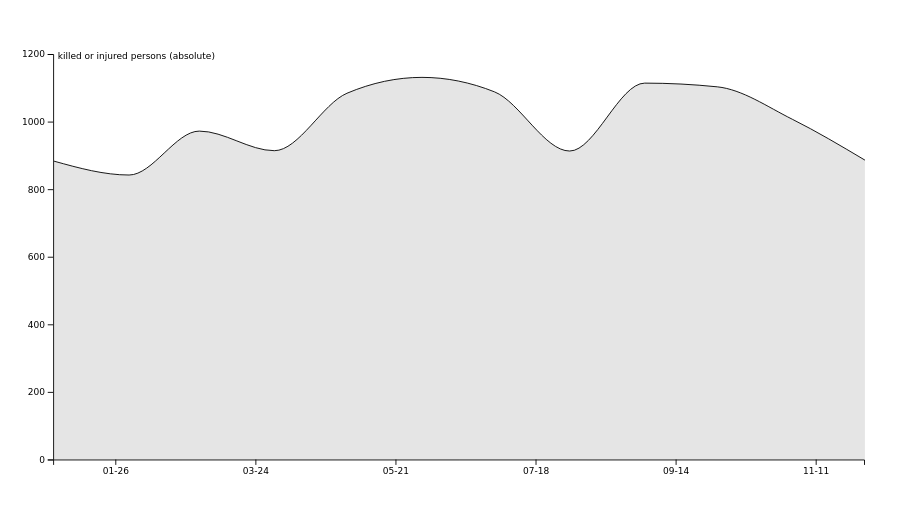
\includegraphics[width=0.9\linewidth]{figures/time-series-2-to-1-killed-or-injured-absolute-by-year-per-month.png}
    \caption{Time series of the number of killed or injured persons per month with a 2:1~aspect ratio, by aggregating across all years~2005--2010.}
    \label{figure-time-series-killed-injured-by-year-per-month}
\end{figure}
An interesting use case for the time series plot is to answer the question whether there is a seasonal influence on the prevalence and severity of road accidents. A citizen living in Paris might ask the following: \enquote{Are roads more dangerous in winter or summer?}
By aggregating injured or killed persons across recent years~(2005--2020) and grouping per month, we get the time series visualization in Figure~\ref{figure-time-series-killed-injured-by-year-per-month}. To be able to spot seasonal trends, we also enable banking to 45\(^\circ\). First, we observe that the monthly number of injured or killed persons is above~800 for all months. But even though one could intuitively think driving in winter would be more dangerous, from December to March there are fewer road casualties.
Because the citizen lives in Paris, they would like to check whether the findings also hold true when only considering accidents from the Paris metropolitan area.
Therefore they switch to the map view to select a grouping by Departements and click on their Departement of Paris. 
With our current implementation this use case faces two difficulties: \Ni because Paris is divided into several Departements, it can be difficult to select the correct Departement from the map and \Nii becuase of the sampling described in Section~\ref{data} the selected sub-set is to small to observe any trends in the time series plot.
In future work, we plan to improve this interaction by optimizing the application code to work with the whole dataset.
Arguably the citizen could also find this seasonal influence in a recursive pattern visualization. But the color mapping of the recursive pattern technique would make it difficult, especially for color-blind people, to distinguish and quantify the extent of seasonality.

\subsection{Prevalence of Woman}
\begin{figure}
    \centering
    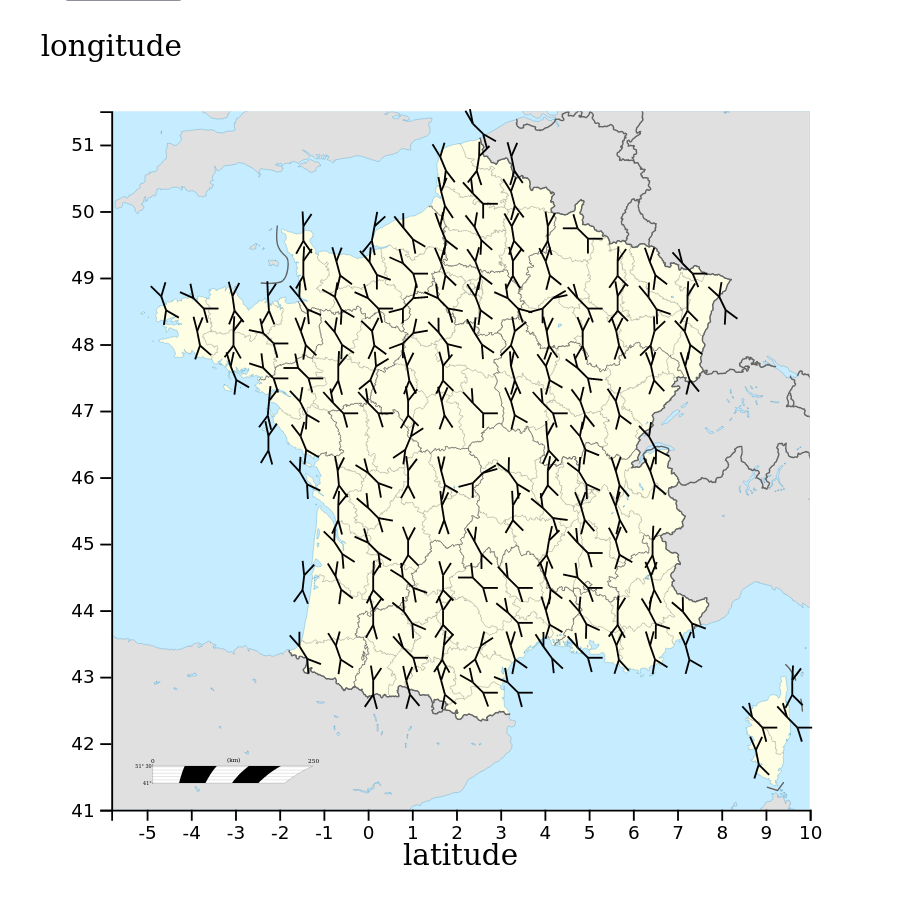
\includegraphics[width=0.6\linewidth]{figures/stick-figures-by-grid-20-20-average.png}
    \caption{Stick figure icons of average person characteristics on a map of France after partitioning the map into a \(20 \times 20\)~grid.}
    \label{figure-stick-figures-grid-average}
\end{figure}
For the second use case, a policy maker would like to answer the question: \enquote{Do women drive more carefully?} They would also like to know if that is true for specific regions in France.
To answer this information need, they open the person characteristics map and select a grouping by a \(20 \times 20\)~grid as shown in Figure~\ref{figure-stick-figures-grid-average}.
Features are aggregated by averaging across the individual persons in each of the 400~grid cells. The resulting stick figures indicate that for most regions in France the majority of participants in road accidents is male, thereby confirming the policy maker's question.
Interestingly however, in some regions there are equally many accidents involving men as there are involving women, especially in coastal regions.
In contrast to other visualization techniques such as Chernoff faces, the stick figures induce a texture on the map, where the rotated figures are visible as a \enquote{flow} from north-west to south-east.
However, other icon-based techniques might work better to emphasize differences in the other 4~plotted dimensions, because with stick figures smaller differences only result in barely noticable angular changes in the stick figure.
In our visualization application this limitation can be avoided by selecting the x-ray stick figure style as then the individual stick figures differ more than with averaging, resulting in greater differences of the stick figure angles.

\subsection{Rainy Nights}
\begin{figure}
    \centering
    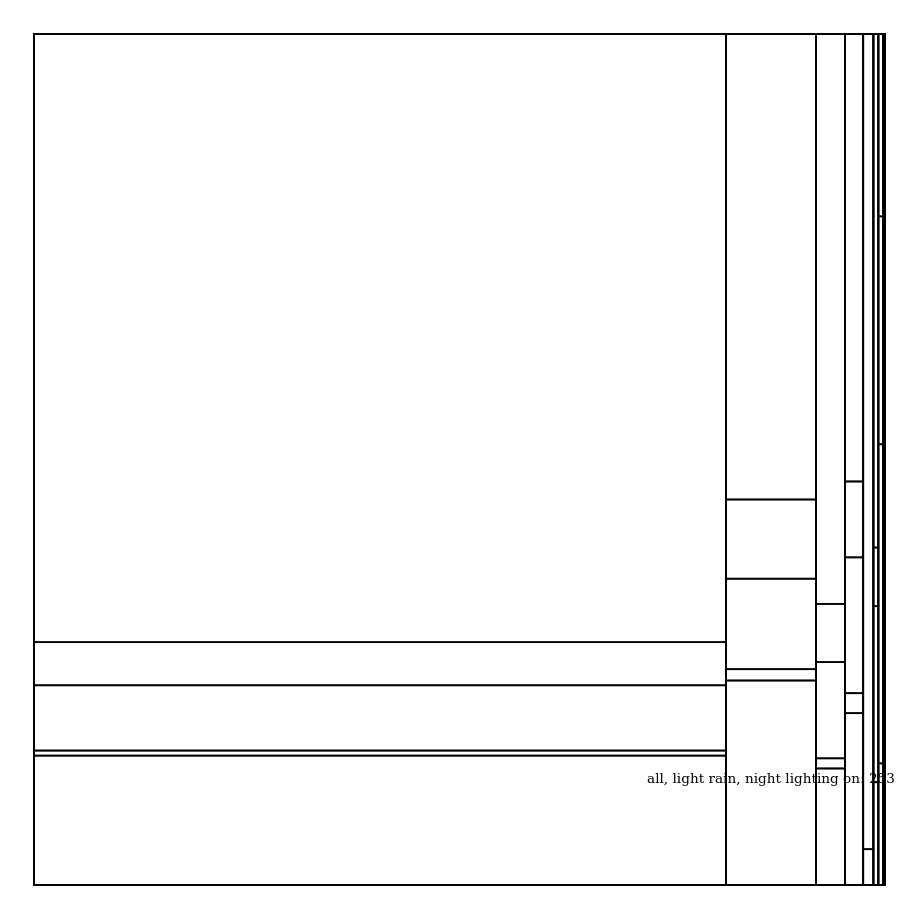
\includegraphics[width=0.6\linewidth]{figures/tree-treemap-weather-light-condition.png}
    \caption{Tree map of accidents by weather and light condition.}
    \label{figure-treemap-weather-light-condition}
\end{figure}
Our last use case is a public infrastudture planner wondering where the current infrastrucure might not suffice in mitigating road accidents. Because they are aware that the majority of accidents occurs under normal conditions~(i.e., with normal weather and in daylight), they would like to identify unexpectedly high numbers of accidents, specifically targetting the public lighting.
This use case is relevant because after decades of development in public infrastructure planning, good starting points for infrastructure projects are not always obvious to find. 
In the treemap visualization they therefore select the weather dimension followed by the light condition dimension.
The resulting treemap is shown in Figure~\ref{figure-treemap-weather-light-condition} and indicates that indeed the majority~(5769~accidents) occur in daylight when the weather conditions are normal.
However, by comparing the number of accidents with public lighting enabled, the treemap indicates that when it rains disproportionately many accidents occur with enabled public lighting. Hence, it would make sense to investigate whether the lights are either too dimmed, leading to limited visibility, or too bright, blinding drivers that pass public lighting.
Even though in this case only three dimensions~(weather, light condition, number of accidents) are visualized, the treemap visualizaiton is still inferior to a scatterplot, because in a scatterplot the number of accidents~(clusters of points in the plot) would not be as easy to interpret as with a treemap node's area.

\section{Related Work}
Geographical plots have already been used in the past to visualize multidimensional data of road accidents.
\textcite{LeLL2020} visualize road traffic accidents in the city of Hanoi, Vietnam from~2015 to~2017, based on data from the Transport Police Department of Hanoi.
For their visualizations they split the 1132~accidents from the small dataset per season and then assign each accident a severity index that is calculated as a weighted sum of the number of light, severe, and fatal accidents~\cite{GeurtsWBV2004}.
For each season and time of day \citeauthor{LeLL2020} then transform accidents into a grid using Kernel Density Estimation~\cite{Anderson2009}. Accidents in this grid are then displayed on a street map of Hanoi where they plot the severity index value per grid cell~(Figure~3 of their paper~\cite{LeLL2020}).
Similar to our work, \citeauthor{LeLL2020} also group the geographically tagged accident records into grid cells of equal size. However, while their grid size is relatively small and dynamically determined~(using a bandwidth of 1\,km for Kernel Density Estimation), our grid is relatively large~(approximately 50\,km). Also, they only encode a single dimension per plotted data point by the point's size while in our visualization multiple dimensions are plotted in stick figure style~\cite{PickettG1988}.
Moreover, the map by \citeauthor{LeLL2020} features information about infrastructure by including street paths and visualizing different types of roads. We did not find a freely available street map of France, and hence only use a simple map that only indicates different Departements inside France. It would be an interesting direction of future research to integrate a map of the French public road network into our visualizations.

\textcite{LavravcJTK2008} also visualize traffic accidents and their seasonality by analyzing a database of 453\,451~accident that occurred in Slovakia from~1995 to~2005.
To indicate seasonal influences on the number of accidents, they propose a two-dimensional heatmap~(Figure~2 of their paper~\cite{LavravcJTK2008}) by months of the year and weekdays. By using a greyscale color coding for the number of accidents they circumvent issues with color-blindness. However, it is even more difficult to visually map from the different shades of grey to the number of accidents by comparing with the plot's legend. Because the shades look so similar, for example, it is nearly impossible to distinguish an accident count of~6001 from~6501.
Neither the visualization by \citeauthor{LavravcJTK2008} nor the visualization by~\citeauthor{LeLL2020} feature user exploration by interactive filtering and changing of visualization styles.


\section{Conclusion and Future Work}
\todo{Fassen sie die Beiträge ihre Visualisierungs-Anwendung zusammen. Wo bietet sie für die Personen der Zielgruppe einen echten Mehrwert?}

\todo{Was wären mögliche sinnvolle Erweiterungen, entweder auf der Ebene der Visualisierungen und/oder auf der Datenebene?}

\section*{Appendix: Git History}
% Generate with: git --no-pager log --all --graph --no-color --date=short --pretty='format:%h%d (%s, %ad)'
% \lstinputlisting[language=,basicstyle=\ttfamily\tiny]{git-log.txt}

\printbibliography

\end{document}

